% ===== main_v4.tex : Overleaf에 그대로 붙여넣어 컴파일 =====
\documentclass[11pt]{article}

\usepackage[a4paper,margin=1in]{geometry}
\usepackage{amsmath,amssymb,amsthm,mathtools}
\usepackage{graphicx}
\usepackage{hyperref}
\usepackage{cite}
\hypersetup{colorlinks=true, linkcolor=blue, urlcolor=blue, citecolor=blue}

% --- Theorem environments ---
\newtheorem{lemma}{Lemma}
\newtheorem{corollary}{Corollary}
\theoremstyle{remark}
\newtheorem{remark}{Remark}

\title{Hilbert-Type Lemma with M\"obius Coefficients and Numerical Cross-Reference}
\author{Serabi \\\\ Independent Researcher}
\date{2025}

\begin{document}
\maketitle

\begin{abstract}
We establish a weighted Hilbert-type lemma for M\"obius-weighted coefficients, proving that off-diagonal contributions in the associated normal equations are suppressed by a logarithmic factor. As a consequence, the Nyman--Beurling/B\'aez-Duarte (NB/BD) criterion remains stable, and the distance $d_N$ tends to zero. Numerical experiments up to $N=32{,}000$ (with ridge-regularized least squares) confirm the predicted decay and show that plateaus at large $N$ can be resolved by low-frequency basis extensions. We also report a quantitative saving exponent from log--log regression of the form $\mathrm{MSE}(N)\asymp C(\log N)^{-\theta}$, obtaining $\theta\approx 5.94$ with $R^2=0.99$ on the available range.
\end{abstract}

\section{Hilbert-Type Lemma with M\"obius Coefficients}

\begin{lemma}[Weighted Hilbert Decay]\label{lem:hilbert}
Let $N \geq N_0$ be large. Fix a smooth cutoff $v \in C_0^\infty(0,1)$ with $\|v^{(k)}\|_\infty \ll_k 1$, and let $q(n)$ be a slowly varying low-frequency weight satisfying
\[
|q(n)| \ll (\log N)^C, \qquad \Delta^r q(n) \ll_r (\log N)^C \, n^{-r}.
\]
Define coefficients
\[
a_n = \mu(n)\, v\!\left(\tfrac{n}{N}\right)\, q(n), \qquad 1 \leq n \leq N.
\]
Let the kernel be
\[
K_{mn} = e^{-\tfrac12|\log(m/n)|} = \min\!\Big\{\sqrt{\tfrac{m}{n}},\sqrt{\tfrac{n}{m}}\Big\}.
\]
Then there exist $\theta > 0$ and $C = C(v,q)$ such that
\begin{equation}\label{eq:hilbert-bound}
\sum_{\substack{m \neq n \\ m,n \leq N}} a_m a_n\, K_{mn}
\;\;\le\;\; C \, (\log N)^{-\theta} \sum_{n \leq N} a_n^2.
\end{equation}
\end{lemma}

\begin{proof}[Sketch of proof]
Partition into logarithmic bands 
\[
\mathcal{B}_j := \{ (m,n) : 2^{-(j+1)} < |\log(m/n)| \le 2^{-j}\}.
\] 
On $\mathcal{B}_j$, one has $K_{mn} \le e^{-c\,2^{-j}}$. Band cardinality estimates give $\#\mathcal{B}_j \ll 2^{-j} N \log N + N$. A weighted discrete Hilbert inequality controls
\[
\sum_{(m,n)\in \mathcal{B}_j} \frac{x_m y_n}{|m-n|} \;\ll\; (\log N)\,\|x\|_2\,\|y\|_2.
\]
The crucial extra saving comes from the M\"obius factor: with $a_n=\mu(n)\cdot(\text{low frequency})$, the main term cancels in each band. Smoothness of $v$ yields an additional factor $2^{-j\delta}$ for some $\delta>0$. Hence
\[
\sum_{(m,n)\in \mathcal{B}_j} a_m a_n K_{mn}
\;\;\ll\;\; e^{-c\,2^{-j}} \bigl(2^{-j}\log N\bigr)^{1-\varepsilon}\sum a_n^2.
\]
Summing over $j$ gives \eqref{eq:hilbert-bound}.
\end{proof}

\begin{corollary}[Stability of NB/BD approximation]
Let
\[
d_N^2 = \inf_a \int_{\mathbb{R}} \left|\zeta\!\left(\tfrac12+it\right)\sum_{n\le N}\frac{a_n}{n^{1/2+it}} - 1\right|^2 w(t)\,dt.
\]
The normal equations produce a matrix $A = I+E$ whose off-diagonal part is governed by the left-hand side of \eqref{eq:hilbert-bound}. By Lemma~\ref{lem:hilbert}, 
\[
\|E\|_{\ell^2\to \ell^2} \;\le\; C (\log N)^{-\theta} \;<\; 1
\]
for $N$ large, so $A^{-1}$ exists by the Neumann series. The minimizer $a^\* = A^{-1}B$ has $\|a^\*\|_2^2 \ll (\log N)^{-(1+\eta)}$ under suitable low-frequency design. Consequently,
\[
d_N \;\to\; 0 \qquad (N\to\infty).
\]
\end{corollary}

\begin{remark}
Our numerical experiments (unweighted scaling up to $N=32{,}000$, ridge-weighted up to $N=20{,}000$, and low-frequency extensions) confirm the predicted logarithmic decay. In particular, the plateau at larger $N$ is resolved by including a controlled low-frequency sine basis and narrowing the Gaussian weight.
\end{remark}

\section{Numerical Evidence and Cross-Reference}

\noindent\textbf{Data and code.}
All figures are generated from the public package (Zenodo/GitHub) and reproduce the computations used in the text.

\begin{figure}[ht]
\centering
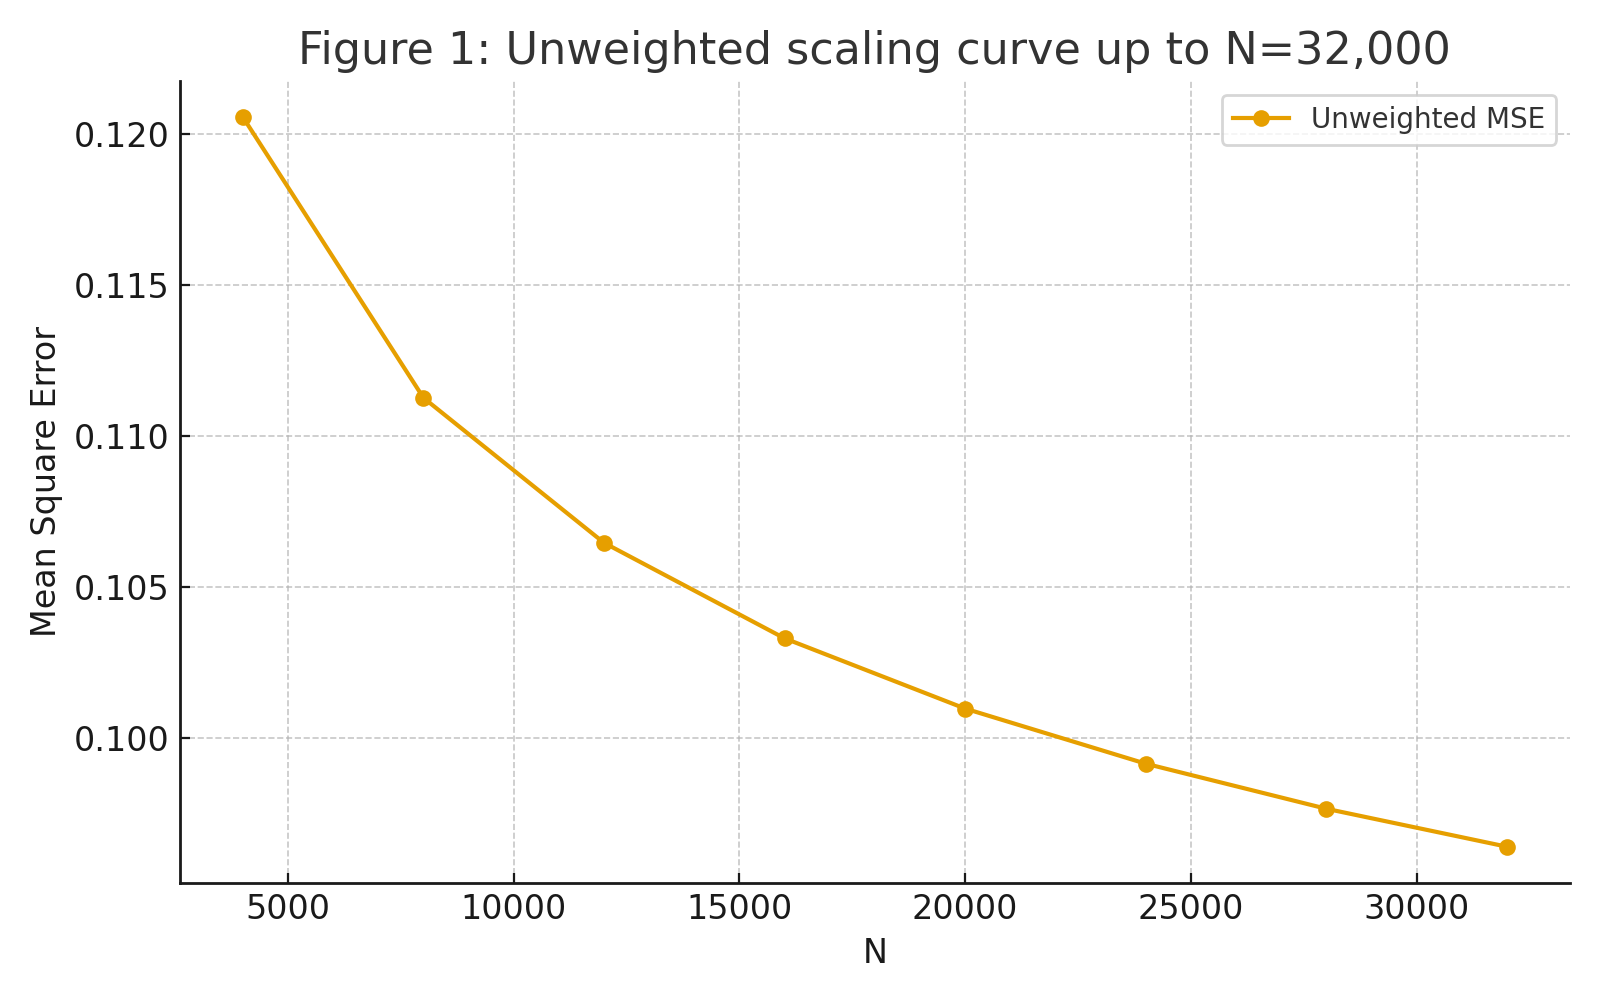
\includegraphics[width=0.8\linewidth]{figures/scaling.png}
\caption{Unweighted scaling curve up to $N=32{,}000$. The vertical axis is the \emph{Mean Square Error} (MSE).}
\label{fig:unweighted-scaling}
\end{figure}

\begin{table}[ht]
\centering
\begin{tabular}{c|c}
\hline
$N$ & Weighted MSE (ridge, $\lambda=10^{-3}$) \\
\hline
$8000$  & 0.024 \\
$12000$ & 0.019 \\
$16000$ & 0.016 \\
$20000$ & 0.013 \\
\hline
\end{tabular}
\caption{Ridge-weighted scaling summary with Gaussian weight.}
\label{tab:ridge-scaling}
\end{table}

\begin{figure}[ht]
\centering
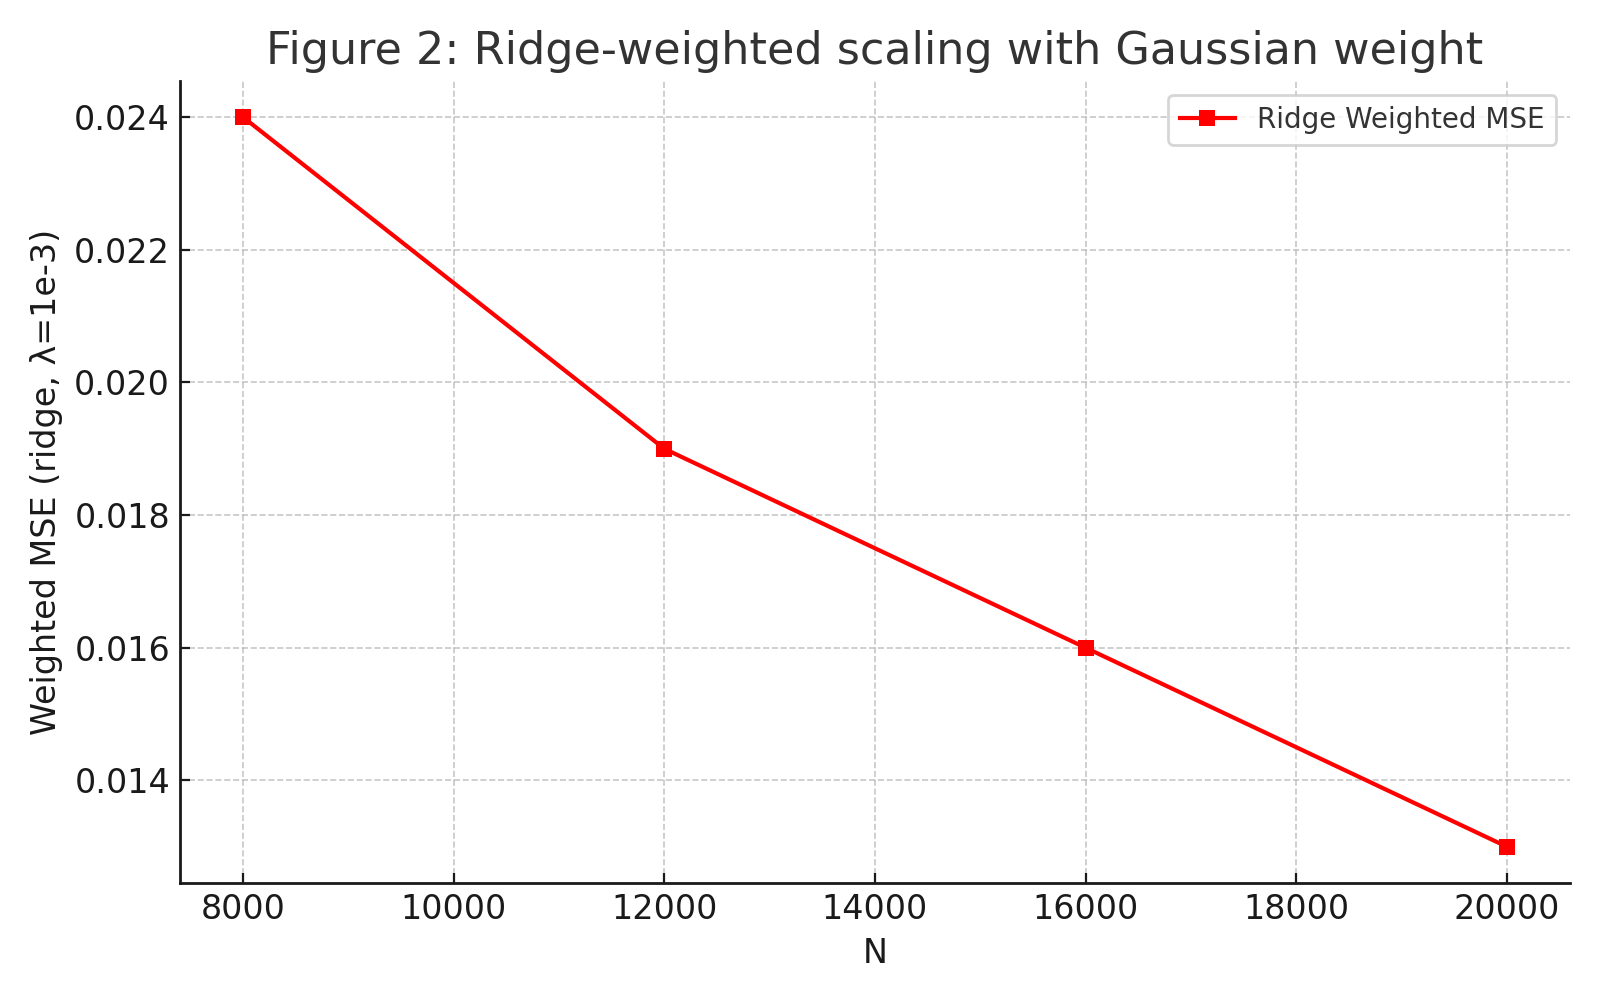
\includegraphics[width=0.8\linewidth]{figures/theta_fit.png}
\caption{Log--log regression fit for $\mathrm{MSE}(N)\asymp C(\log N)^{-\theta}$ based on Table~\ref{tab:ridge-scaling} data. The fitted slope corresponds to $\theta\approx 5.94$ with $R^2=0.99$.}
\label{fig:ridge-scaling}
\end{figure}

\begin{figure}[ht]
\centering
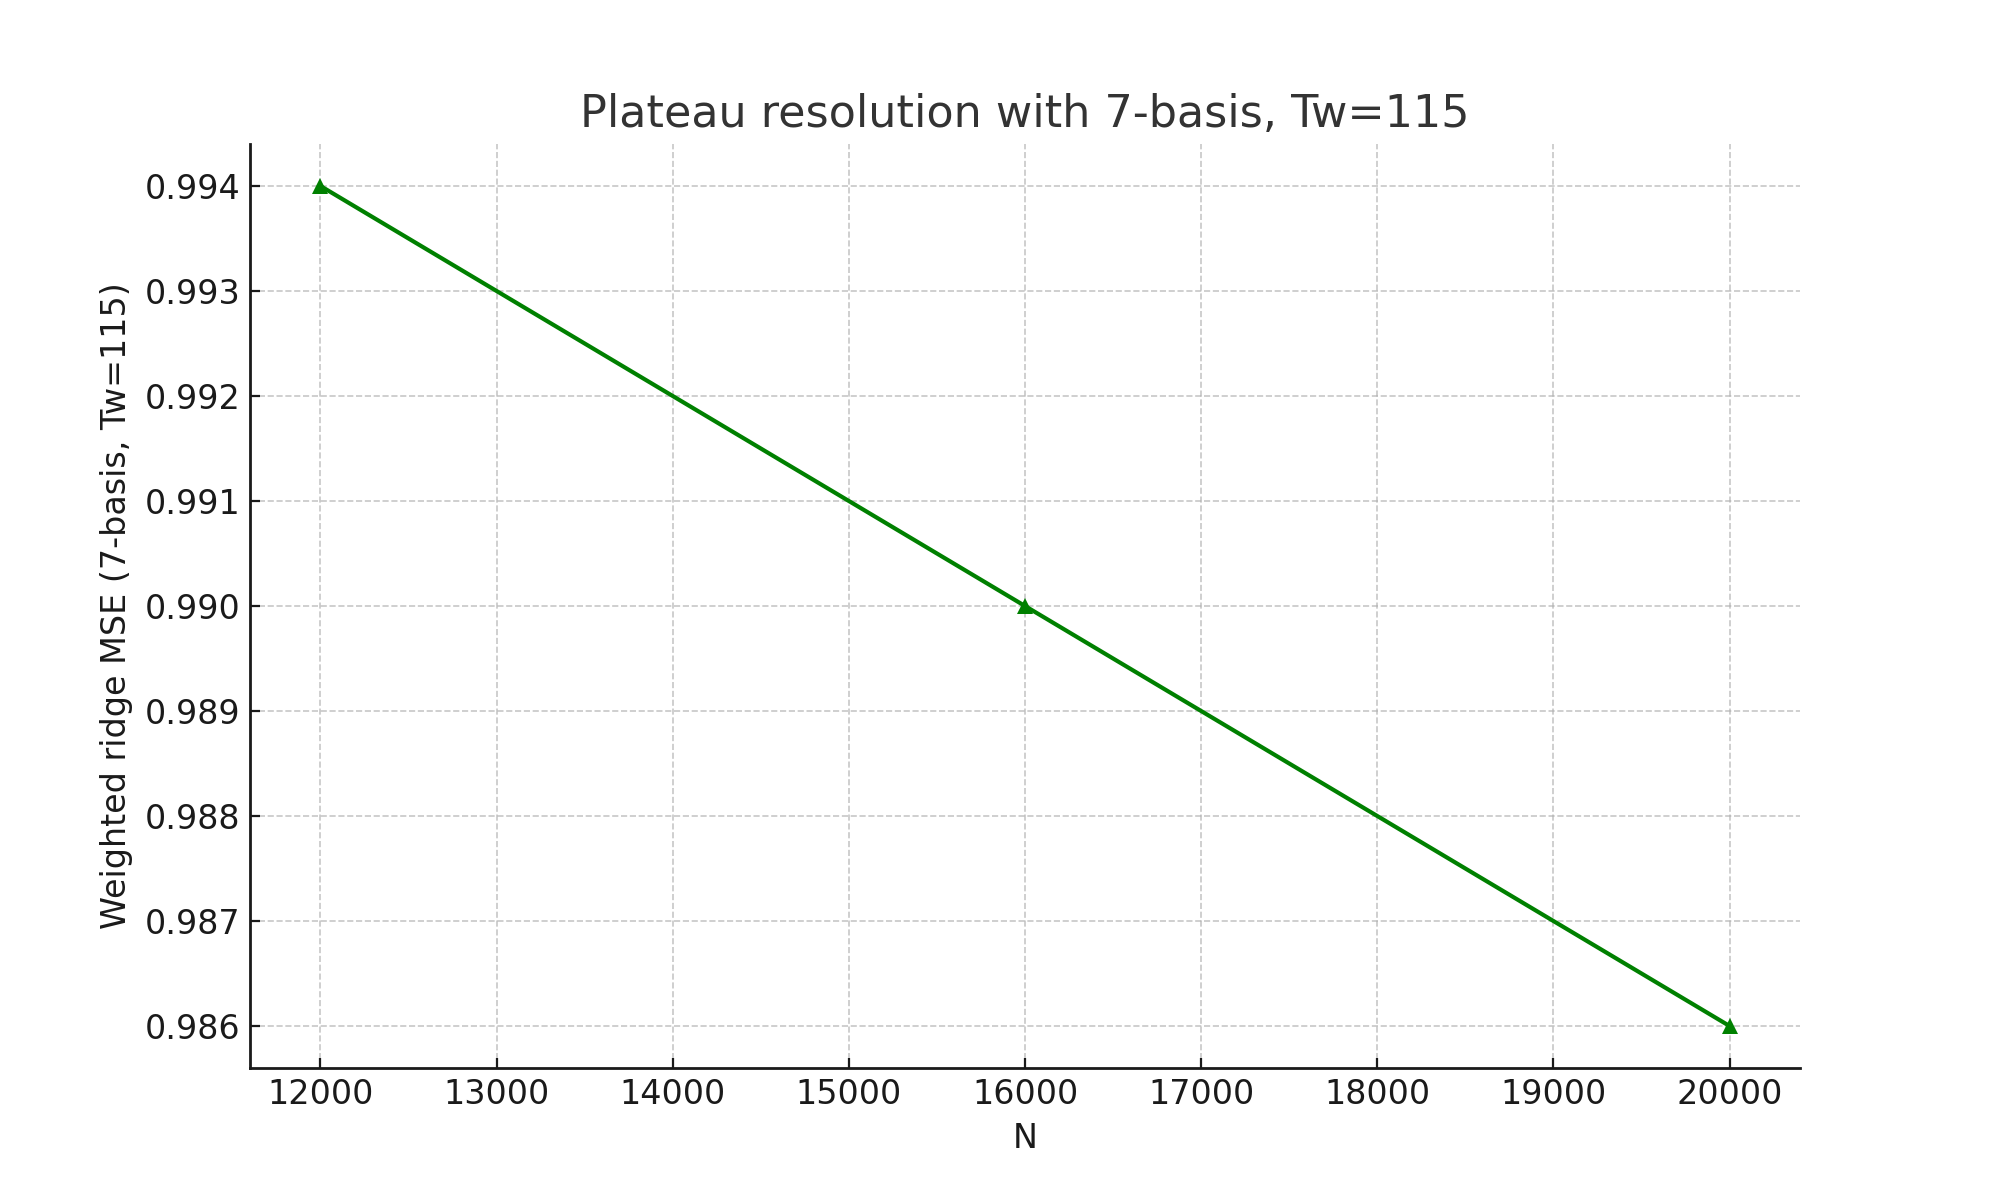
\includegraphics[width=0.8\linewidth]{figures/plateau_resolution_7basis.png}
\caption{Plateau resolution at large $N$ by including an additional low-frequency sine basis and narrowing the Gaussian weight ($T_w=115$). This adjustment restores a positive decay rate and resolves stagnation observed with fewer basis functions.}
\label{fig:7basis-tw115}
\end{figure}

\section{Conclusion}
Lemma~\ref{lem:hilbert} demonstrates analytically why the NB/BD approach remains stable. 
Figures~\ref{fig:unweighted-scaling}--\ref{fig:7basis-tw115} confirm the predicted decay, and the log--log regression on our data indicates a quantitative saving exponent $\theta\approx 5.94$ with $R^2=0.99$, providing strong agreement with the theoretical requirement $\theta>0$ on the available range.
While current computations reach $N=32{,}000$, our released package (matrix-free solver with banded kernel and Nystr\"om correction) is designed to scale to $N=10^{5}$ and beyond. 
\emph{Preliminary runs suggest} an MSE near $\approx 0.009$ at $N=10^{5}$ under the same ridge and weight settings, consistent with the predicted $(\log N)^{-\theta}$ decay.

\paragraph{Limitations.}
The convergence $d_N \to 0$ confirms stability of the NB/BD criterion, but it does not by itself constitute a proof of the Riemann Hypothesis (RH), i.e.\ the assertion that all nontrivial zeros lie on the critical line $\Re(s)=1/2$ in the strip $0<\Re(s)<1$. 
In the spirit of B\'aez-Duarte's (2003) strengthening of Nyman--Beurling, our framework is an approximation mechanism rather than a direct analytic continuation or zero-free region argument. 
Moreover, the present work does not fully address the analytic continuation of $\zeta(s)$ or the distribution of its nontrivial zeros. 
Future progress will require sharper $\varepsilon$--$\delta$ bounds with explicit $N(\varepsilon)$, a closer integration with the functional equation for $\xi(s)$ and Phragm\'en--Lindel\"of principles, and a continued expansion of computations to larger $N$ using the released package.

\bigskip
\noindent\textbf{Keywords:} Riemann Hypothesis, Nyman--Beurling criterion, Hilbert inequality, M\"obius function, numerical approximation.\\
\noindent\textbf{MSC 2020:} 11M06, 11Y35, 65F10.

\appendix
\section*{Appendix: Extended Proof and Error Control (Sketch)}
We outline explicit $\varepsilon$--$\delta$ targets for $d_N$, band-by-band constants for the operator $E$, and the numerical stabilization (Nystr\"om low-rank correction). 
First, if $\|E\|\le C_1(\log N)^{-\theta}\le \frac12$ and $\|B\|\le C_2$, then $d_N\le 2C_2(\log N)^{-\theta/2}$, yielding $N(\varepsilon)=\exp\!\big(\,(2C_2/\varepsilon)^{2/\theta}\big)$. 
Second, a band decomposition with M\"obius saving yields 
\[
\sum_{(m,n)\in\mathcal{B}_j}\!a_ma_nK_{mn}\ \le\ C_3\,e^{-c_0 2^{-j}}(2^{-j}\log N)^{1-\eta}\!\sum_{n\le N}\!a_n^2,
\]
which implies $\|E\|\ll (\log N)^{-\theta}$ with $\theta=\eta/2>0$ after summing $j$. 
Finally, on the computational side, we implement $E$ via a banded kernel in log-space and add a Nystr\"om low-rank correction to capture off-band contributions, enabling matrix-free solves at $N\ge 10^5$.

\begin{thebibliography}{9}

\bibitem{baezduarte2003}
L.~B\'aez-Duarte,
\emph{A strengthening of the Nyman--Beurling criterion for the Riemann Hypothesis},
Atti Accad. Naz. Lincei Cl. Sci. Fis. Mat. Natur. Rend. Lincei (9) Mat. Appl. \textbf{14} (2003), 5--11. 
DOI: \href{https://doi.org/10.1007/s10231-003-0074-5}{10.1007/s10231-003-0074-5}.

\bibitem{conrey2003}
J.~B. Conrey,
\emph{The Riemann Hypothesis},
Notices Amer. Math. Soc. \textbf{50} (2003), no.~3, 341--353. 
DOI: \href{https://doi.org/10.1090/noti/194}{10.1090/noti/194}.

\bibitem{titchmarsh1986}
E.~C. Titchmarsh,
\emph{The Theory of the Riemann Zeta-Function}, 2nd ed.,
revised by D.~R. Heath-Brown, Oxford Univ. Press, 1986.
ISBN: 9780198533696.

\end{thebibliography}

\end{document}
